\documentclass{article}
\usepackage{ison2022,amssymb,amsmath,epsfig}
\setcounter{page}{1}
\ninept
\graphicspath{{pics/}}

\title{Our current ISon template}

%\name{Thomas Template}
%\address{Formular Group \\
%Documenttown, Paperbourg\\
%{\tt template@formular.net}}
%
% uncomment above lines and comment out following lines for
% the twoauthors template.
\twoauthors{Tina Template}
	{Formular Group \\ Documenttown, Paperbourg\\ {\tt template@formular.net}} {Francois Formatted}
{Second Institute \\ Address \\ {\tt
your.email@add.ress}}

\begin{document}
\maketitle
%
\begin{abstract}
We generated this LaTeX template by a mild adaptation of the ICAD proceedings template. The template is also highly similar to AES16th, WASPAA'97, WASPAA'99 and ICASSP'99 templates and aims at producing conference proceedings in electronic form. The format is essentially the one used for ICASSP conferences.

Please use either LaTex or the Word format to prepare the submission.
Submit your paper in pdf format.

The easiest way is to use pdflatex. Alternatively you may compile using latex, create a ps file using dvips and a pdf file using ps2pdf...

\end{abstract}
%
\section{Introduction}
This is the template for the ISon 2022 meeting.
This is the template for the ISon 2019 meeting. This is the template for the ISon 2016 meeting. This is the template for the ISon 2013 meeting. This is the template for the ISon 2010 meeting. 
%
\subsection{Figures}
Here an example for a figure
\begin{figure}[ht]
\centerline{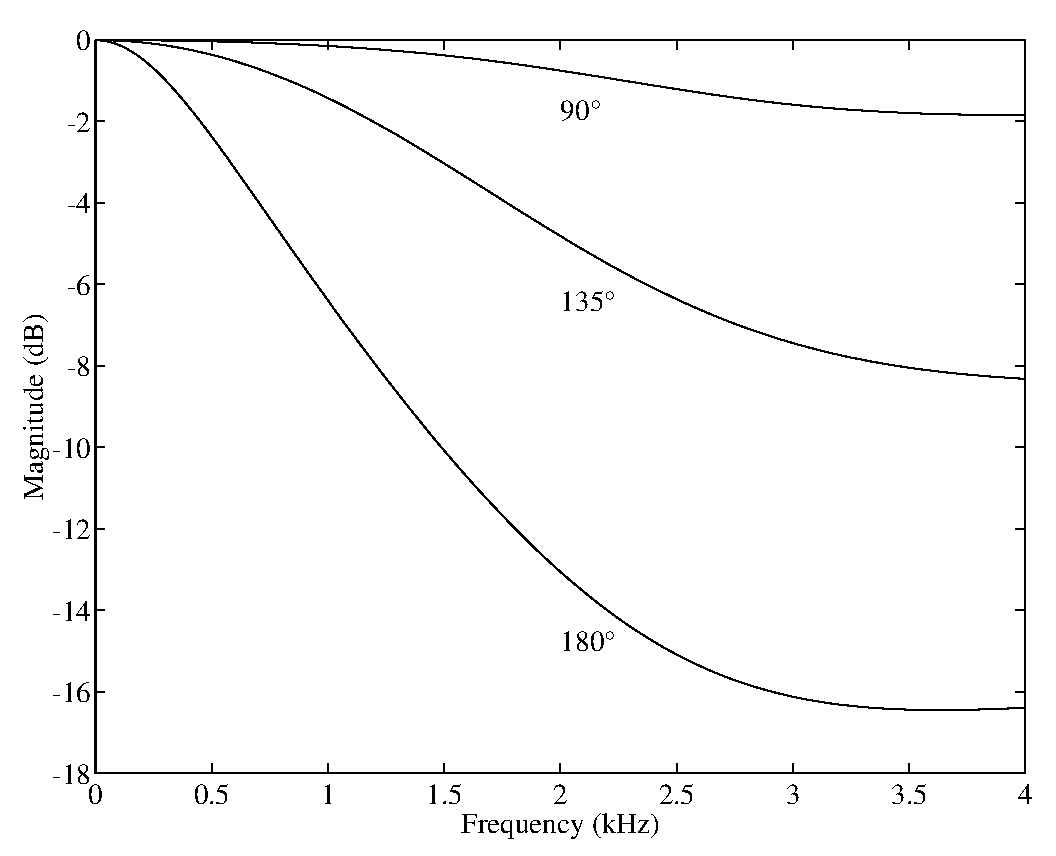
\includegraphics[width=75mm]{dir}}
\caption{{\it Directivity measurement of a trumpet.}}
\label{iresp}
\end{figure}
%
%\newpage
\subsection{Equations}
Equations should be placed on separate lines and numbered:

\begin{equation}
x(t) = s(f_\omega(t))
\label{eq1}
\end{equation}
where \(f_\omega(t)\) is a special warping function
\begin{equation}
f_\omega(t)=\frac{1}{2\pi j}\oint_C \frac{\nu^{-1k}d\nu}
{(1-\beta\nu^{-1})(\nu^{-1}-\beta)}
\label{eq2}
\end{equation}
A residue theorem states that
\begin{equation}
\oint_C F(z)dz=2 \pi j \sum_k Res[F(z),p_k],
\label{eq3}
\end{equation}
Applying theorem \ref{eq3} to \ref{eq1},
it is quite straightforward to see that
\begin{equation}
1 + 1 = \pi
\label{eq4}
\end{equation}
%
\subsection{Page numbers}
Page numbers will be added to the document electronically, so
{\em please leave the numbering as is}, that is, the first page will be
ISon2022-1 and the last page will be, e.g., ISon2022-6.

\subsection{Citing}
Follow IEEE instructions for citations. Use short citations~\cite{icad1,ison1}.
%
\section{Conclusions}
write a conclusion...

\bibliographystyle{IEEEbib}
\bibliography{references}

\end{document}
